\documentclass[onecolumn]{revtex4}

%Language&Font
%\setmainfont{Times New Roman}
%\usepackage{lmodern} 
%\usepackage[T1]{fontenc}
\usepackage[english]{babel}
%========================================
%Pictures
\usepackage{pgfplots}
\usepackage{graphicx}
\graphicspath{{img/}}
\DeclareGraphicsExtensions{.pdf,.png,.jpg,.eps}
%========================================
%Title
%\title{TlXSe2 Report}
%\author{A> Nosenko A.}
\date{\today}
%========================================
%Table contents

%========================================

\begin{document}
\maketitle
\tableofcontents
\section{Band structure: insight from DFT computations}
\subsection{Computational details}

First principles calculations are used for the investigation of the electronic properties of TlEr$_2$Se$_2$ and TlTm$_2$Se$_2$. 
Ab initio calculations were performed using the pseu
dopotential projector-augmented wave method \cite{Kresse1999} implemented in the Vienna ab initio simulation package
(VASP) \cite{Kresse1996,Kresse1993} with an energy cutoff of 700 eV for the plane wave basis set. A $\Gamma$-centred  28x28x28 k-point mesh was used to sample the Brillouin zone. Spin-orbit coupling effects were included self-consistently. We used the experimental low-temperature crystal structure to initialize our
computations from Materials project database \cite{MaterialsProject}. The $ f $-electrons of Er and Tm were treated as core electrons. Nonmagnetic configuration were chosen. Post-processing produced with pymatgen python library \cite{Pymatgen}. 
 
\section{Results}
Fig. 1 shows the and structure and the density of states (DOS) in TlEr$_2$Se$_2$. The top of the valence band is set at zero energy and the scale is in electron volt. As the valence band maxima and the conduction band minima lies on the $T$ and the point between the $F$ and $\Gamma$ points [ARTEM, pls look at the correspondence band and dos. Minima in band is lower than in DOS *fixed]. Hence, this shows the indirect band gap nature in TlEr$_2$Se$_2$. The value of the gap is 1ev [ARTEM in band -- 0.9 pls check. *fixed] 
When Er is replaced by Tm, the band gap is similar to the previous case, as shown in Fig. 2. 
The top of the valence bands in both materials consists predominantly from $ p $-states of Se.
The conduction band electrons originated both from the orbitals of $ d $  electrons of Er(Tm) and $ p $  electrons of Tl.  
 
 

%\begin{figure}[ht]
%	\centering
%%	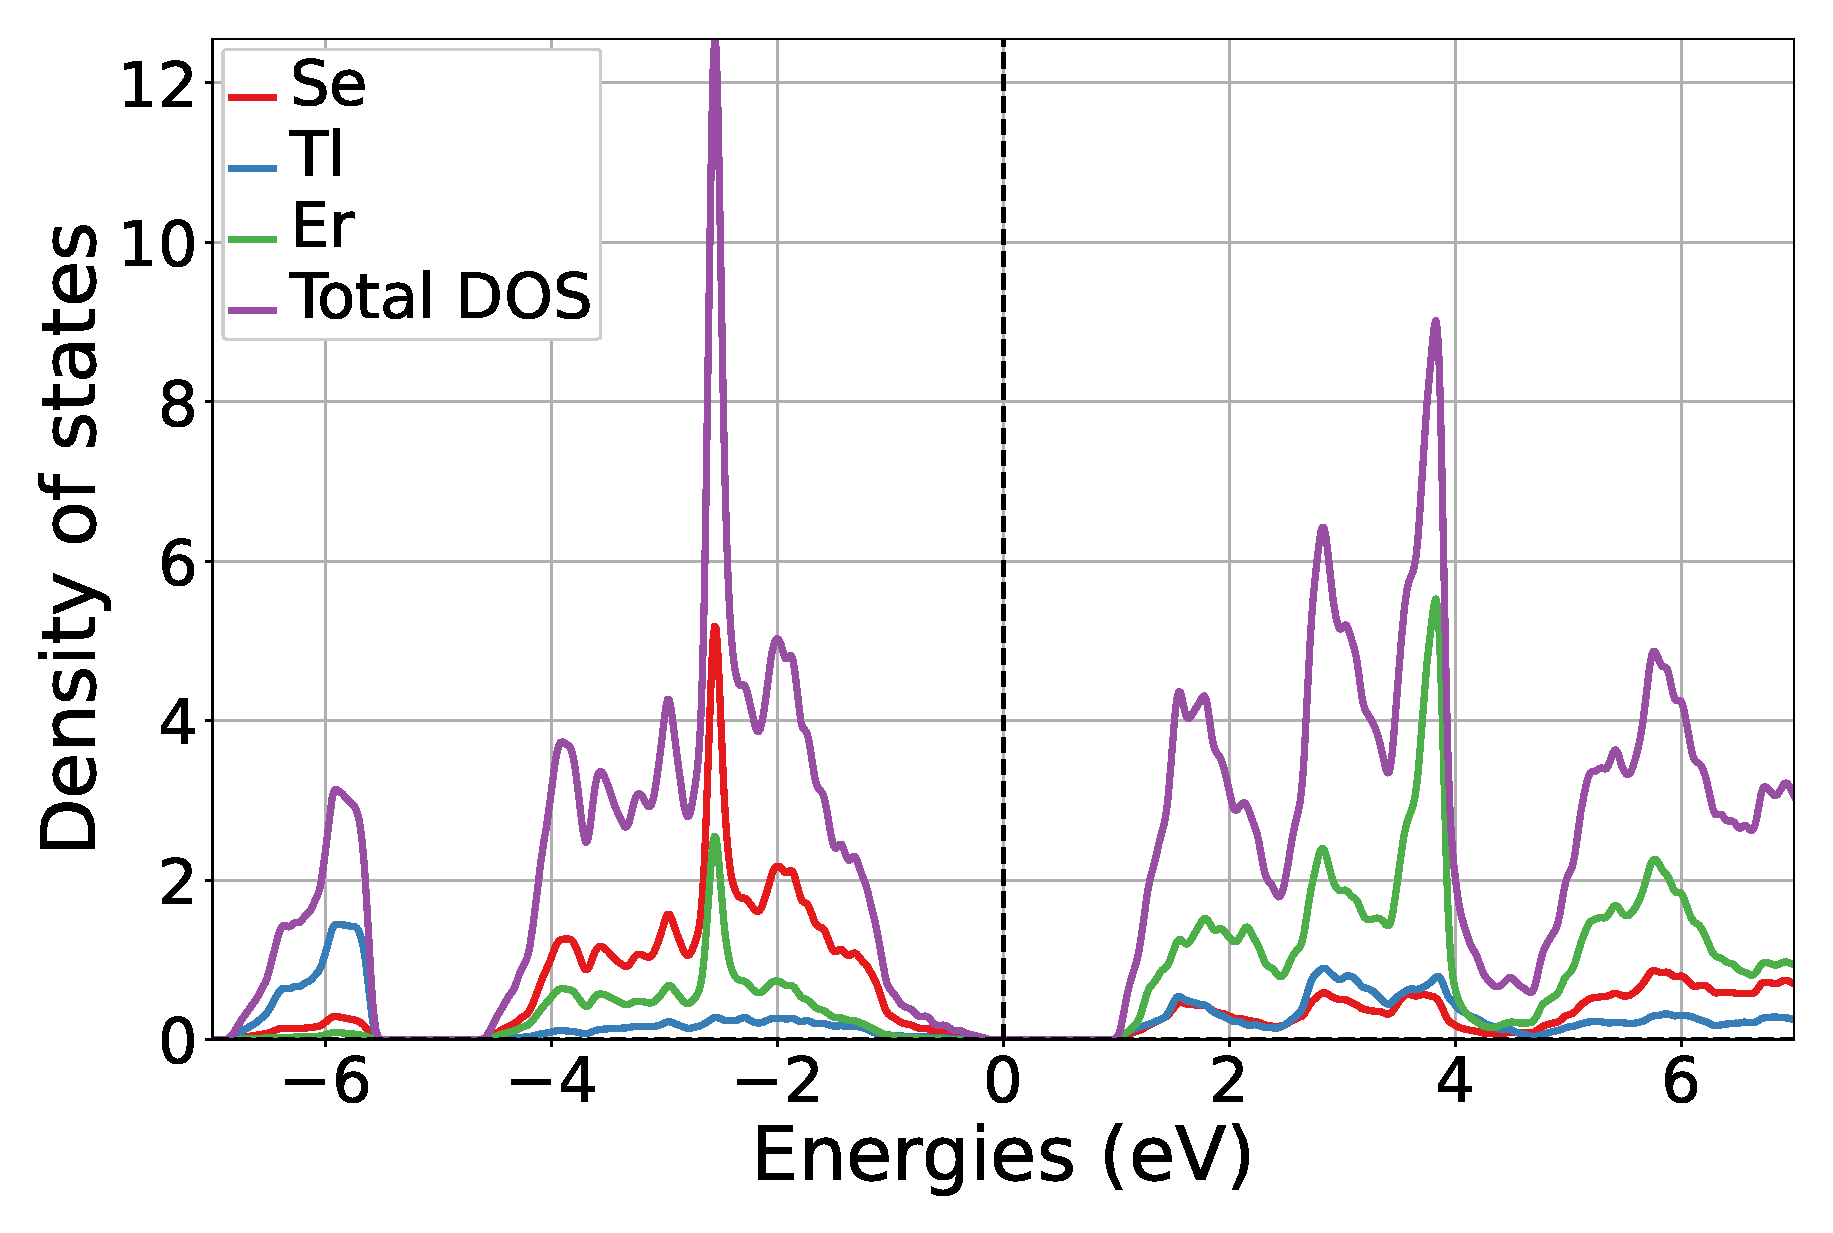
\includegraphics[scale=0.4]{img/Er_DOS}
%	\caption{dos}
%\end{figure}
%\begin{figure}[ht]
%	\centering
%	\includegraphics[scale=0.4]{Er_BAND-eps-converted-to}
%	\caption{band}
%\end{figure}
\begin{figure}[ht]
	\centering
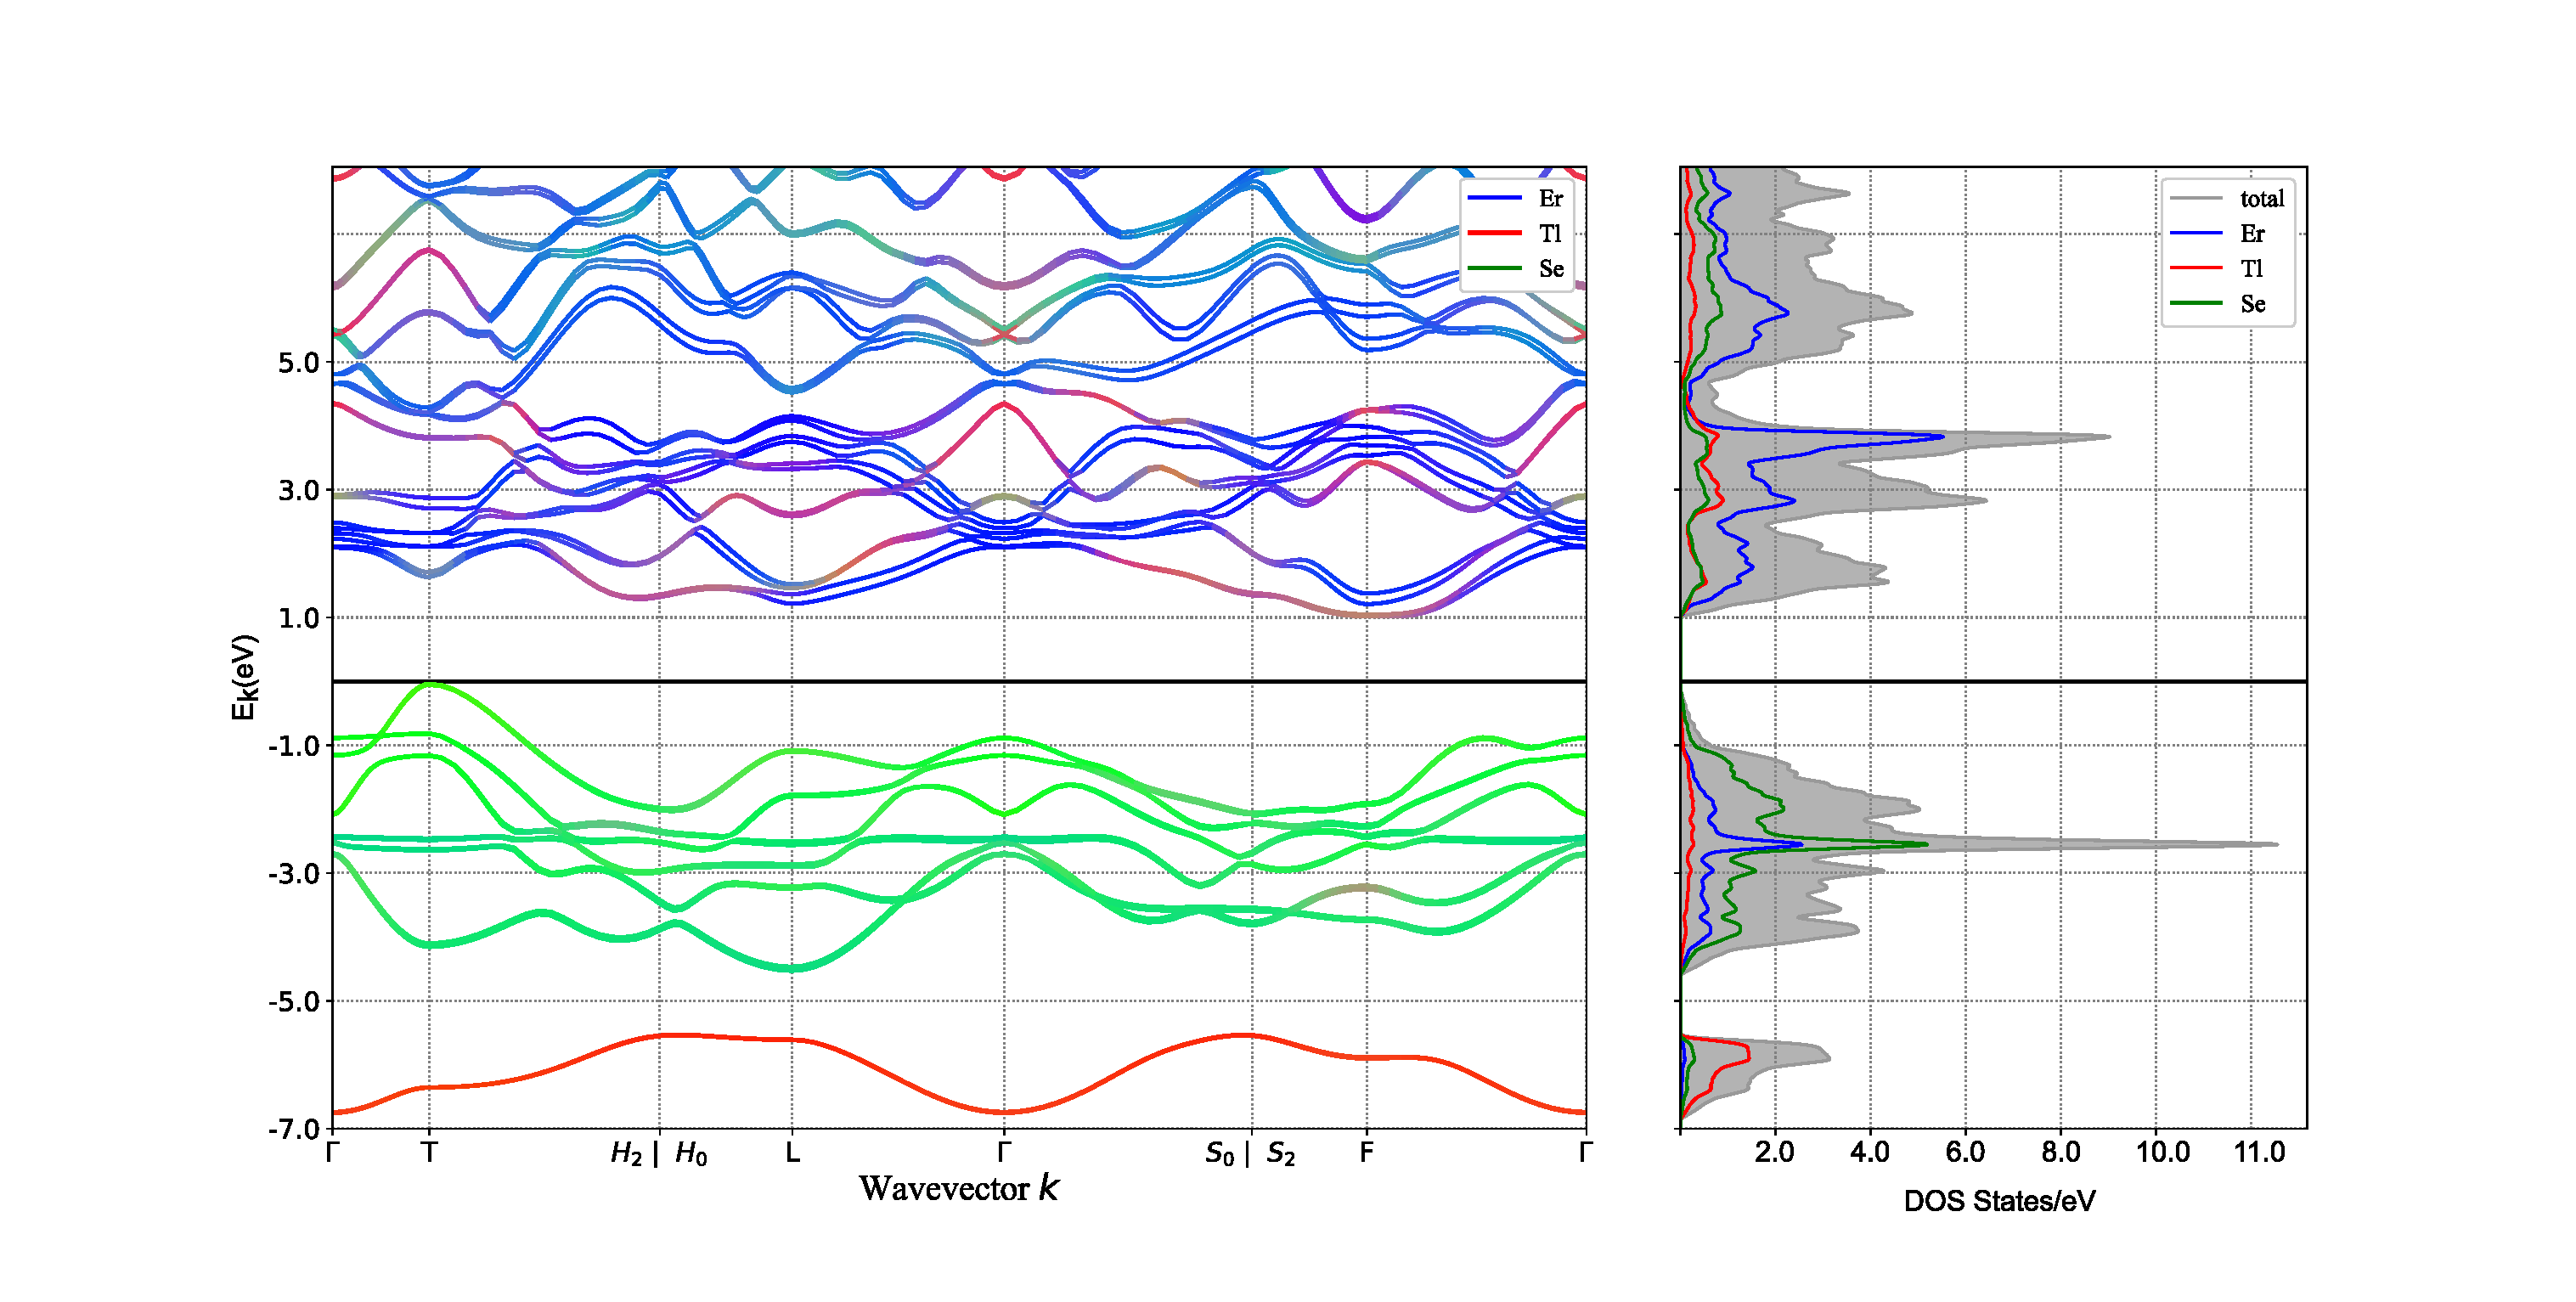
\includegraphics[scale=0.4]{img/Er_BAND+DOS}
	\caption{Band structure and density of states of TlEr$_2$Se$_2$. }
\end{figure}	
\begin{figure}[ht]
	\centering
	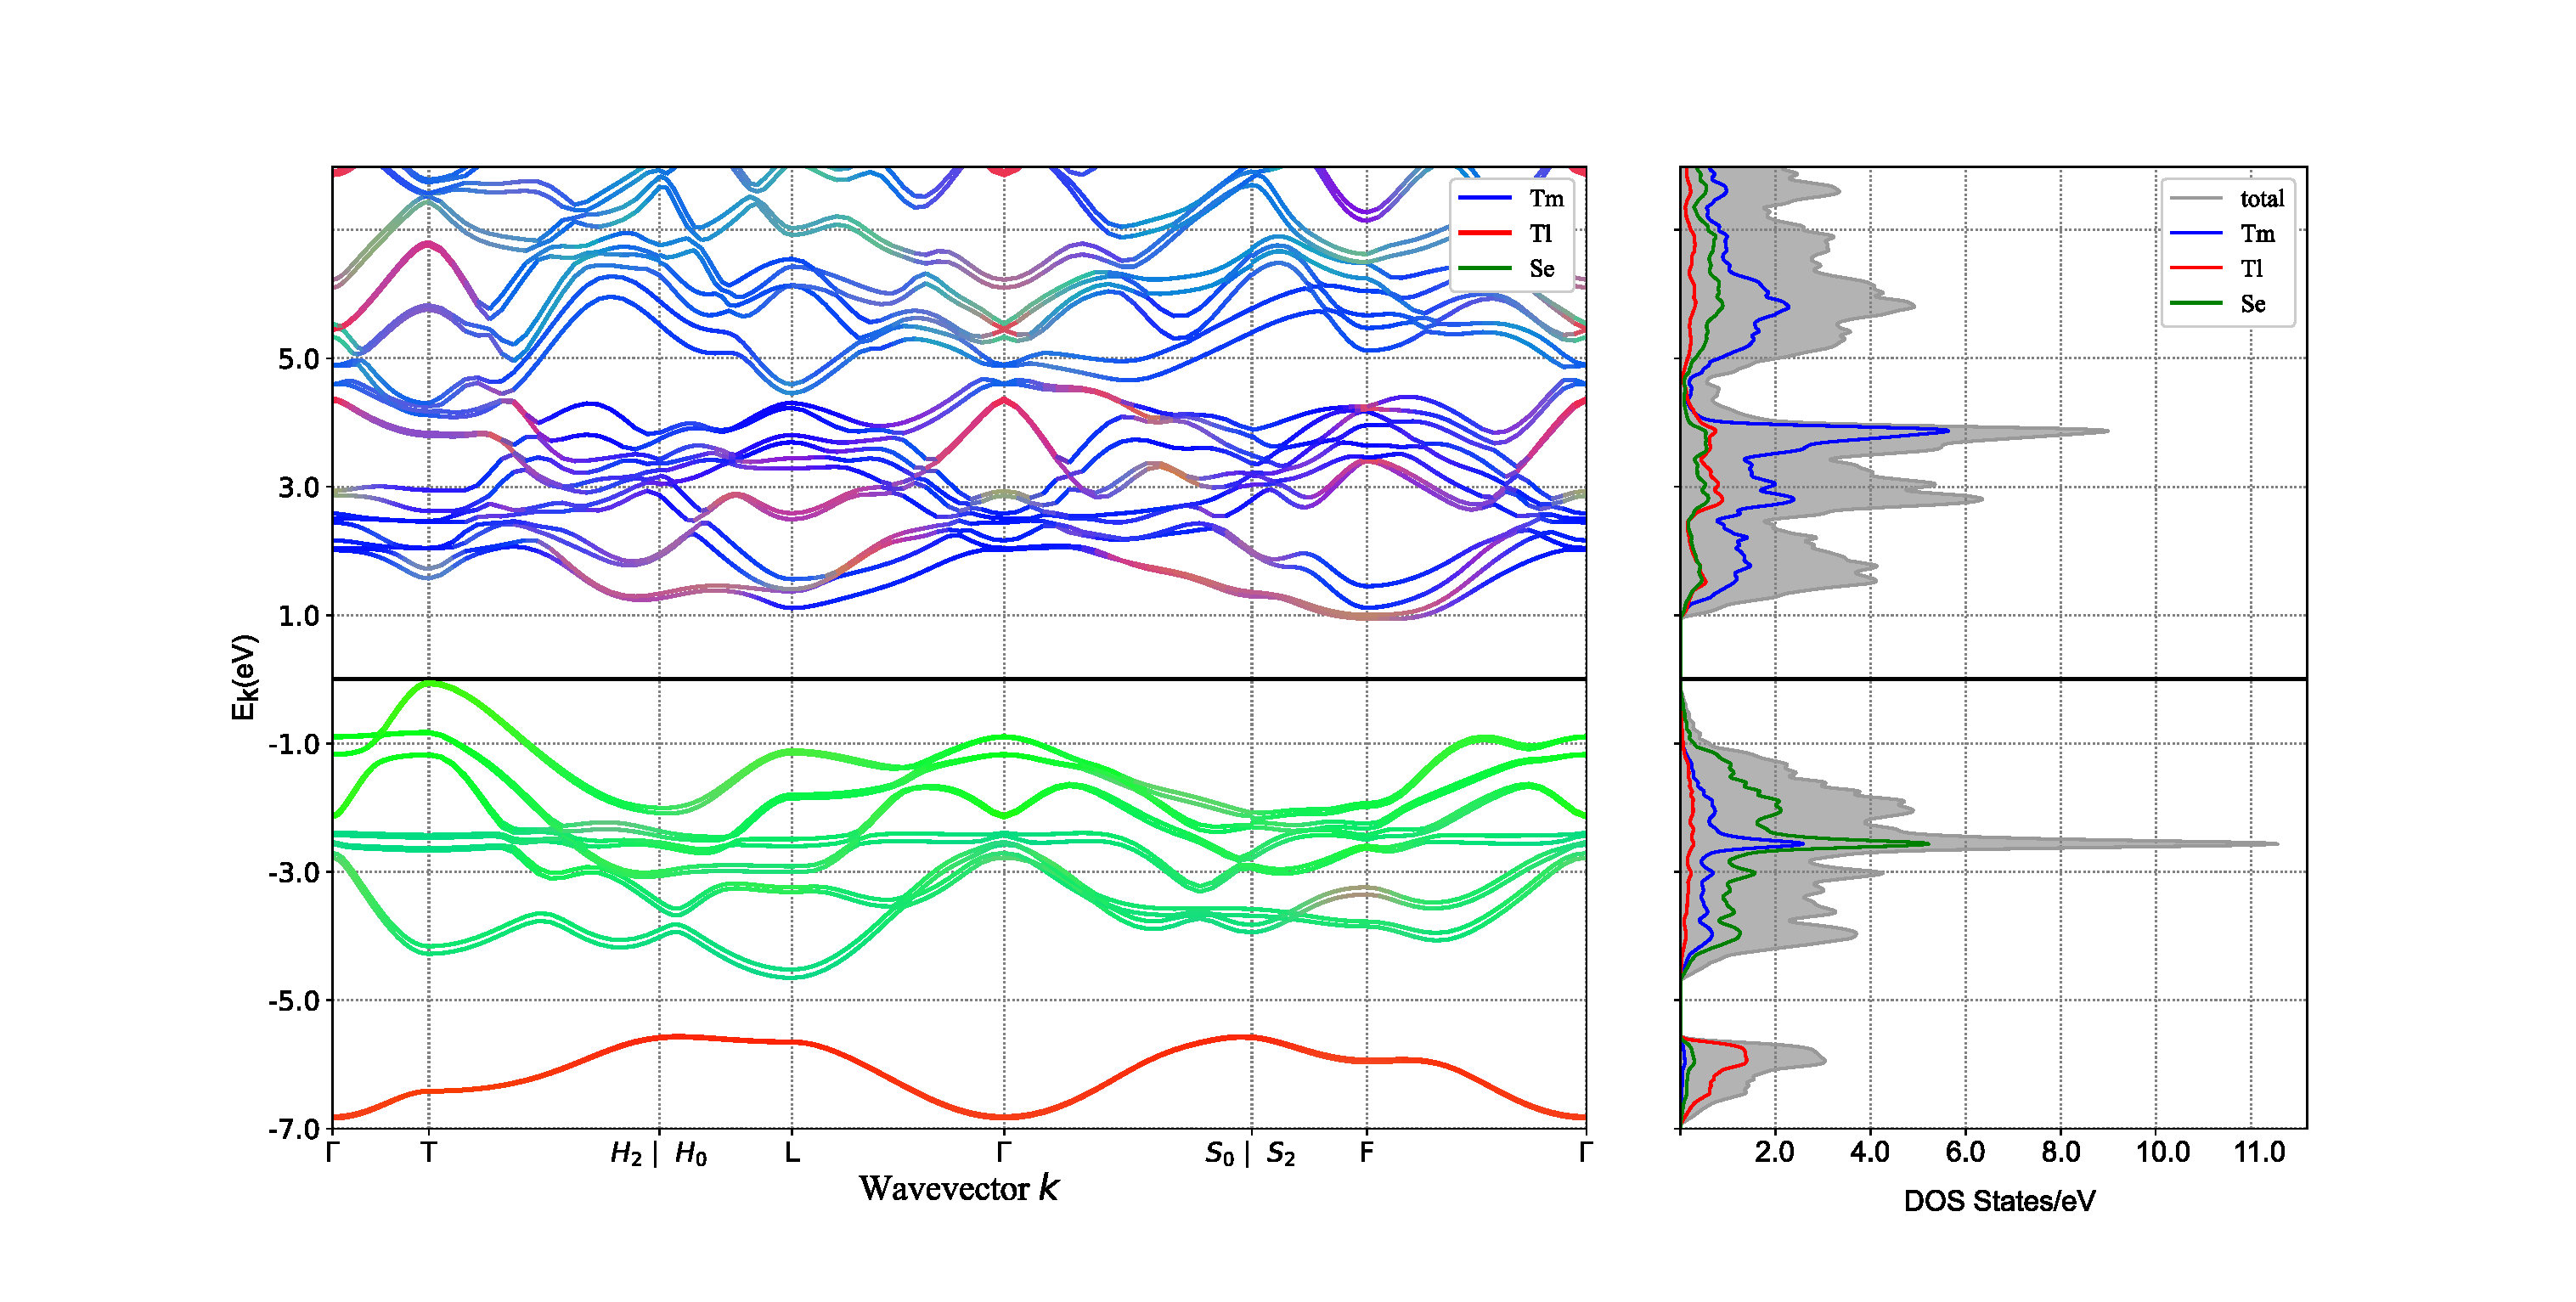
\includegraphics[scale=0.4]{img/Tm_BAND+DOS}
	\caption{Band structure and density of states of TlTm$_2$Se$_2$. }
\end{figure}
%\include{Er_res.tex}
%\include{Tm_res.tex}

\begin{thebibliography}{99}
\bibitem{Kresse1999} G. Kresse and D. Joubert, Physical Review B \textbf{59}, 1758 (1999)
\bibitem{Kresse1996}G. Kresse and J. Furthm\"{u}ller, Physical Review B  \textbf{54}, 1011169 (1996)
\bibitem{Kresse1993}G. Kresse and J. Hafner, Physical Review B \textbf{48}, 13115 (1993).
\bibitem{Pymatgen} Ong, Shyue Ping, William Davidson Richards, Anubhav Jain, Geoffroy Hautier, Michael Kocher, Shreyas Cholia, Dan Gunter, Vincent L. Chevrier, Kristin A. Persson, and Gerbrand Ceder, Computational Materials Science \textbf{68}, 101936 (2013)
\bibitem{MaterialsProject} Jain, Anubhav and Ong, Shyue Ping and Hautier, Geoffroy and Chen, Wei and Richards, William Davidson and Dacek, Stephen and Cholia, Shreyas and Gunter, Dan and Skinner, David and Ceder, Gerbrand and Persson, APL Materials \textbf{1}, 011002 (2013)
\end{thebibliography}


\end{document}